\chapter{Introduction}
\section{Executive Summary}

Software security is a collective activity that involves producers and consumers of code, open source maintainers, security teams, and organisation leadership.
The same impediments that hinder agility and quality - different workflows, poor collaboration, lack of visibility - also make it difficult to build software securely.
Existing security tools are not designed to solve this problem - they are designed to extract value from a broken model.

GitHub is in a unique position to address this challenge. As the home of open source, we are already in the supply chain of most companies. We understand the code, the data, and the people involved. Customer conversations make it clear they believe we are uniquely positioned to secure open source. With our increased role in the end-to-end DevOps toolchain we are also well placed to help secure TMR’s development practices and proprietary code.

\begin{itemize}
  \item \mintinline{c}|in line code snippet in C | - Lorem Ipsum
  \item \mintinline{c}|in line code snippet in C | - Lorem Ipsum
\end{itemize}

\newpage

\section{Background}

Illustrated in Figure \ref{fig:devsecops} is DevSecOps.

\lipsum[1-2]

\begin{figure}[h]
  \centering
  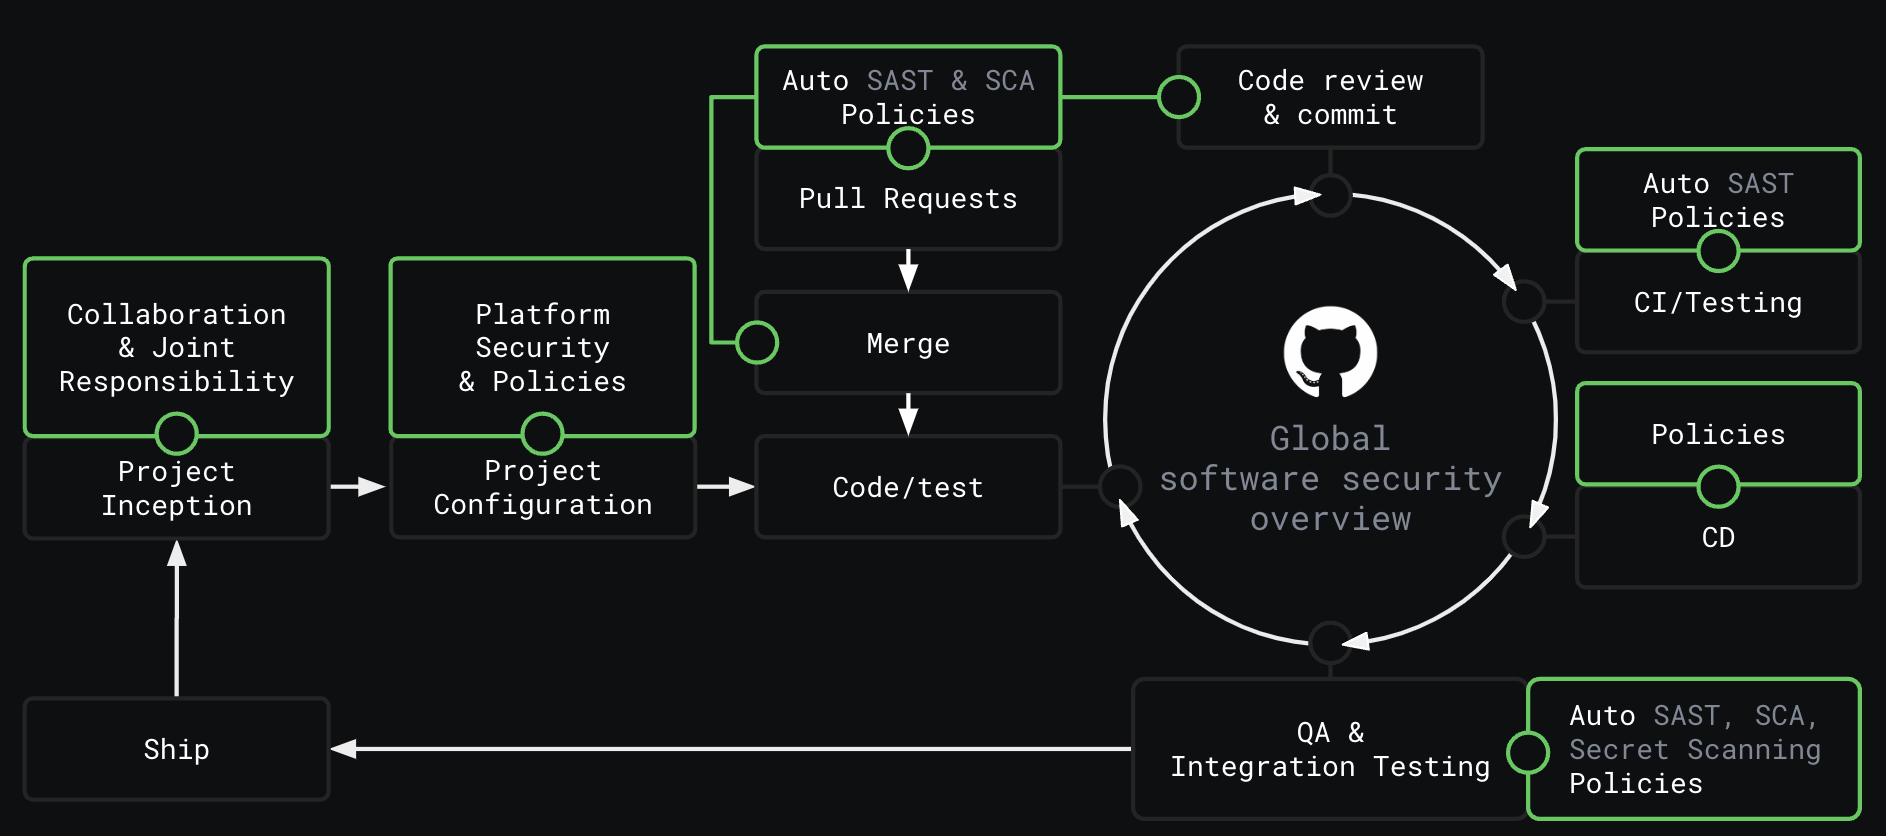
\includegraphics[width=\textwidth]{devsecops}
  \caption{Insert your caption here}
  \label{fig:devsecops}
\end{figure}


